
We train and assess our method using the protein decoy datasets from
the CASP competition \cite{moult2014critical}.  We use the CASP7 to
CASP10 data as training set and the CASP11 data as test set, for a
total of 564 target structures in the training set and 83 target
structures in the test set. Each target from the training set has 282
decoys on average.
%
The test dataset is split into two subsets \cite{kryshtafovych2015}:
``stage~1'' with 20 decoys per target selected randomly from all
server predictions, and ``stage~2'' with the 150 decoys per target
considered best by the Davis-QAconsensus evaluation
method \cite{kryshtafovych2015}.
%
The native structures were not included in the analysis, neither
during the training phase nor during the testing phase. To make the
structural data more consistent, the side chains of all decoy
structures were optimized using the SCWRL4 program
\cite{krivov2009improved}.

Training and test datasets cover the same interval of sequences
lengths (see Fig.~S1 in Supporting Information). To ensure that the
training and test sets are significantly different, we have aligned
all test sequences against all training sequences using
blastp \cite{altschul1990basic}.  Less than 11\% of the targets in the
test set (9 out of 83) have sequence similarity with any target in the
training set (see Table~S1 in Supporting Information).

To further assess the similarity of the two datasets, we have computed
their overlap in terms of Pfam families \cite{finn2016pfam}. Pfam
families were found using HMMER \cite{finn2015hmmer} with an E-value
cutoff of 1.0 \cite{finn2016pfam}.  Accounting for targets for which
no Pfam family could be determined, approximately 25\% of the test set
targets share a family with approximately 10\% of the training set
targets (see Table~S2 in Supporting Information).

We have also compared the structures in the training and test sets
using the ECOD database \cite{cheng2014ecod}. This database provides a
five-level classification of all structures of the RCSB PDB
\cite{berman2000protein} according to the following criteria:
architecture (A-group), possible homology (X-group), homology
(H-group), topology (T-group), and family (F-group).  Since the ECOD
classification is domain-based, multi-domain protein chains can belong
to multiple A-, X-, H-, T-, or F-groups.  The higher the level two
protein domains occupy, the more structurally similar they are.
%
A summary of the overlap between the training and test sets is
presented in Fig.~\ref{Fig:summaryTable}. For each target domain in
the test set (T0759 to T0858), a black tile indicates that at least
one structure from the training set belong to the same ECOD group (A,
X, H, T, and F). (See Fig.~S2 in Supporting Information for another
representation of the overlap between the test and training sets.)

\begin{figure}[H]
    \makebox[\textwidth]{
    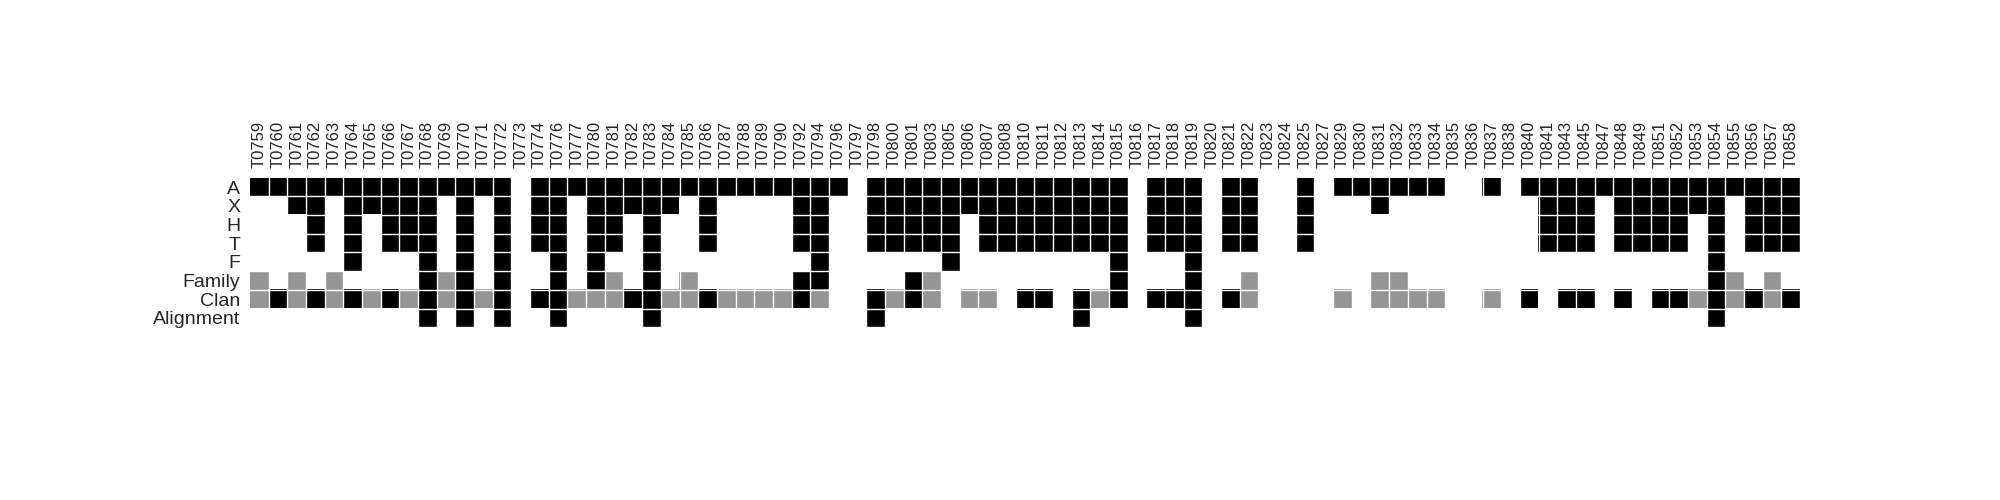
\includegraphics[width=\paperwidth]{Fig/summary_table.eps}
    }
%
    \caption{Overlap of the training set on each target domain of the
    test set (from T0759 to T0858). The first 5 rows of tiles
    correspond to the ECOD classification of protein domains (A-, X-,
    H-, T-, and F-groups). A black tile in any of these rows indicates
    that at least one structure from the training set belongs to the
    same ECOD group as the target. A white tile indicates that no
    structure belongs to the same group. Targets for which no ECOD
    classification is available are left empty (grey).
%%% GL: I see that all targets excluded from the analysis have an
%%% empty row of squares. Is T0838 excluded as well? What about the
%%% targets that are not in the list? (775, 778, 779, 791, 793, 795,
%%% 799, 802, 804, 809, 826, 828, 839, 842, 844, 846, 850) Were they
%%% all excluded from the CASP competition? The CASP11 QA paper
%%% mentions that the following targets were cancelled by the
%%% organizers: 778, 779, 791, 809, 842, 844, 846, 850. What about the
%%% other ones?
    A black tile in the ``Family'' row indicates that at least one
    structure from the training set belongs to the same Pfam family as
    the target. (Grey indicates that no Pfam family information is
    available for the target.) The ``Clan'' row shows similar
    information for Pfam clans. A black tile in the ``Alignment'' row
    indicates that at least one sequence in the training set aligns to
    the target sequence with an E-value smaller than $10^{-4}$. (Grey
    indicates that ??????)}
%%% GL: You're using the code black=yes, white=no, grey=NA. I've
%%% modified the caption to reflect that.
%
    \label{Fig:summaryTable}
\end{figure}
